\section { Design }

\subsection{Audio Effects Data Structure}
The user will likely want to adjust the order of audio effects at will, and as the same time, it must be very fast to insert and  remove audio effects so as to minimise the time spent not processing audio (even a very short pause may result in "crackles" on weaker hardware). To solve this problem, the audio effects can be stored in a linked list, as unlike std::vectors (dynamic C++ arrays) they prove fast insertion, deletion and re-ordering.

\paragraph{}
To satisfy the requirements of multithreading (see below), I will write my own custom "atomic linked list", backed by a mutex\footnote{
	A mutex is an object that prevents multiple threads from accessing data at the same time. It can be thought of as a lock, which can only be unlocked for one thread at a time. They are preferable to spinlocks as they do not require the CPU to waste cycles waiting for the data to be "unlocked", as instead the thread can suspend itself until the mutex becomes available.
}, which will function just like a normal linked list but be thread-safe in all its operations.

\subsection{Multithreading}
In order to maximise ease-of use, the software should have a graphical user environment (GUI) so that the current audio being played can be easily visualised (in-line with objective 2).

\paragraph{}
The program will use a multithreaded model, with a separate "audio thread" and "GUI thread", allowing the two to run concurrently without blocking each other's processing.

\begin{figure}[h]
	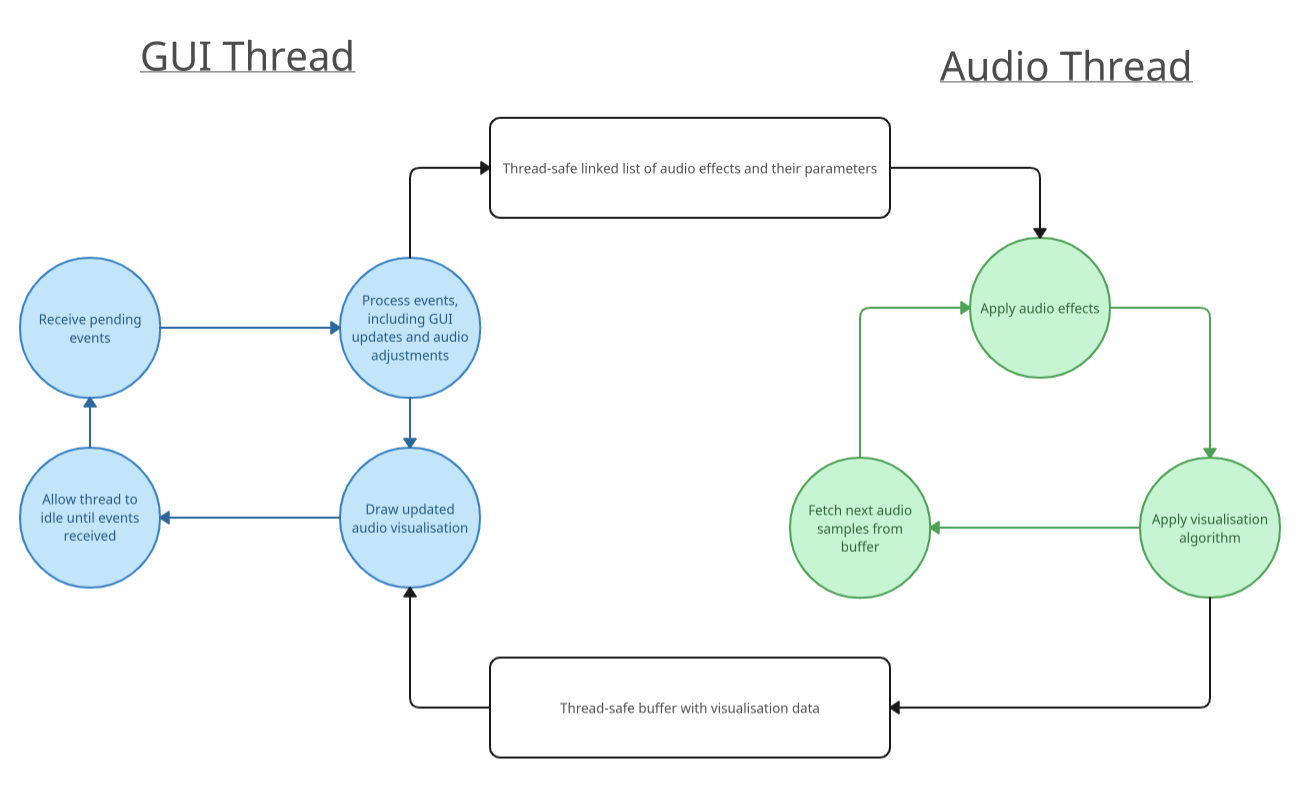
\includegraphics[width=17cm]{threading}
	\caption{Inter-thread diagram}
\end{figure}

\paragraph{}
Typically, GUI programs are written using an event-based paradigm that minimises CPU idle-time. The consequence of this is that, for most of the time, the GUI thread is suspended, awoken only when events from the user (such as mouse clicks or resizing the window) "wake it up". This is desirable in order to minimise system resources used, as more CPU-time will be available for the audio processing requirements, helping to reach the real-time requirements of objective 6. However, this presents a unique challenge. With a single-threaded model:
\begin{itemize}
	\item If the event-based model is followed, the GUI thread is only active when there are pending GUI events to be processed, meaning audio processing can only occur sporadically (resulting in "non-constant" audio)
	\item If instead the GUI thread is constantly active processing audio it will never reach a point where it can process pending events, meaning the program will hang and refuse to process inputs.
\end{itemize}

Hence it is desirable to split the program into two distinct threads - the "audio thread" and the "GUI thread". The audio thread can play the audio and perform all necessary processing tasks, whilst the GUI thread can relay input parameters and commands to the audio thread (such as "switch song", "apply effect", etc.).

\paragraph{}
To avoid race conditions\footnote{
	 Race conditions occur when one thread tries to read data whilst the other writes to it. If, for example, the GUI thread removed an audio effect from the audio effect list (see section 2.1) and freed it from memory whilst the audio thread was applying that same effect, the audio thread would suddenly be reading from invalid memory, likely resulting in a crash or undefined behaviour.
}, the data that is read by both threads should be thread-safe - only one thread should be able to access the data at a time. This can be achieved by using mutexes\footnote{See above footnote on mutexes}.

